%========================================================================================%
%					NOTE
%========================================================================================%
% Probably this theme will not compile with standard pdftolatex compiler due to lack of some 
% fonts used in the theme. It is recommended to compile with XeLaTex instead.

% !TEX program = xelatex

%========================================================================================%
%					DOCUMENT SETUP
%========================================================================================%
\documentclass{beamer} 
\usetheme[progressbar=frametitle]{metropolis}

\usepackage{textpos}

\usepackage{amsmath}

\usepackage{mathrsfs}


%For making diagram and drawing
% \usepackage{tikz}
% \usetikzlibrary{shapes,arrows, fit, positioning}

%For appendix
\usepackage{appendixnumberbeamer}


\usepackage[export]{adjustbox}

%Some additional graphcs tools
\usepackage{graphicx}
%\usepackage{datatool}
%\usepackage{animate}

% For someone using the pgfplot tools
%\usepackage{pgfplots}
%\usepgfplotslibrary{dateplot, groupplots}
%\pgfplotsset{compat=1.14}
%\usepgfplotslibrary{fillbetween}

%Remove words break, wrap instead
\usepackage[none]{hyphenat}


%for custom date
\usepackage[english]{babel}
\usepackage[nodayofweek,level]{datetime}

\usepackage{xspace}
\newcommand{\themename}{\textbf{\textsc{metropolis}}\xspace}

\renewcommand*{\arraystretch}{1.2}

\usefonttheme[onlymath]{serif}




%===================================================================================%
%				FRONT PAGE
%===================================================================================%
\titlegraphic{%
\hfill%

\includegraphics[height=1.5cm, valign=c]{logos/ccfd3.png}%
\hspace{15pt}%

\includegraphics[height=1.5cm, valign=c]{logos/symbol-PL.pdf}%
}

\title{Introduction to concurrency in modern C++}
\date{\vspace{5pt}\formatdate{24}{1}{2022}}
\author{Jakub Gałecki}

%===================================================================================%
%				THEME COLORS
%===================================================================================%
% specify main colors which are being used by the theme
\definecolor{bordercolor}{HTML}{002699}
\definecolor{fillcolor}{HTML}{002699}

% fix theme black color which affects tikz plots
\definecolor{black}{RGB}{0,0,0}




%===================================================================================%
%				ACTUAL DOCUMENT CONTENT
%===================================================================================%

\begin{document}

\maketitle

%force to add logos to the each frame title
\addtobeamertemplate{frametitle}{}{%
\begin{textblock*}{100mm}(.9\textwidth,-0.9cm)

\includegraphics[height=0.8cm, valign=c]{logos/ccfd3_white.png}\hspace{10pt}
\includegraphics[height=0.78cm, valign=c]{logos/symbol-PL-white.pdf}
\end{textblock*}}

\begin{frame}{Disclaimer}
\begin{enumerate}
\item This will be a fire hose talk
\item We are only going to scratch the surface
\end{enumerate}

\includegraphics[width=\linewidth]{firehose.png}
\end{frame}

\begin{frame}{Motivating example}
\begin{itemize}
\item Hashing a vector of strings
\item String comes in
\item Magic happens
\item 64 bit unsigned integer comes out
\item Let's take a look at the serial code...
\item This seems easy to parallelize. What could go wrong?
\end{itemize}
\end{frame}

\begin{frame}{Multithreading}
\begin{itemize}
\item Concurrency: when tasks start, run, and complete in overlapping time periods
\item Parallelism: when two or more tasks execute simultaneously
\item How do we get there? Start a new thread for each task?
\item Lets try to design a task system...
\end{itemize}
\end{frame}

\begin{frame}{Multithreading}
\begin{center}
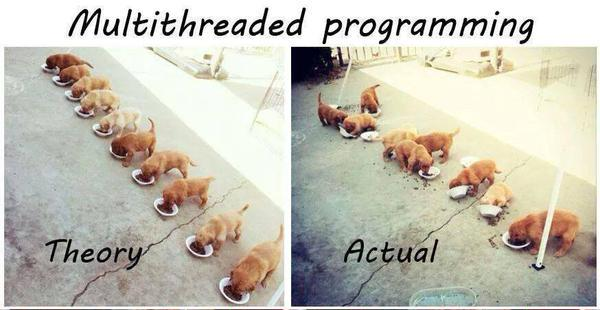
\includegraphics[width=0.8\linewidth]{concurrency.jpeg}
\end{center}
\end{frame}

\begin{frame}{Task Queue}
\begin{itemize}
\item Task = Callable + Arguments
\item Task queue stores tasks and executes them in FIFO order on a thread pool
\item API:
\begin{itemize}
\item push(f, args...)
\item complete()
\end{itemize}
\item Assume single producer for simplicity
\item Use futures to query the completion of individual tasks (outside the scope of this talk)
\item Performance!
\item Let's take a look at Sean Parent's talk for some inspiration...
\end{itemize}
\end{frame}

\begin{frame}[standout]
The features...
\end{frame}

\begin{frame}{Variadic templates}
\begin{itemize}
\item Lets us write templates with an unspecified number of parameters
\item Syntax: \texttt{template < typename ...T >}
\item The above can be instantiated with any number of types (including zero)
\item \texttt{T} is a parameter pack and must be expanded whenever used
\end{itemize}
\end{frame}

\begin{frame}{Perfect forwarding}
\begin{itemize}
\item When writing a function taking arguments by lvalue or rvalue reference, you need to write 2 functions
\item When writing a function \textit{template} taking arguments by reference, we can avoid this by using perfect forwarding
\item Universal reference: \texttt{T\&\&}, where \texttt{T} is a function parameter
\item Use \texttt{std::forward} to pass as lvalue (do nothing) or rvalue (move)
\end{itemize}
\texttt{template < typename T >}\\
\texttt{void fun(T\&\& a) \{}\\
\hspace{0.5cm}\texttt{bar(std::forward<T>(a));}\\
\texttt{\}}
\end{frame}

\begin{frame}{\texttt{std::function}}
\begin{itemize}
\item Type-erased function wrapper
\item Template syntax: \texttt{std::function<R(Args...)>}
\item Wraps arbitrary function object which takes arguments of types \texttt{Args...} and returns \texttt{R}
\item API: docs
\end{itemize}
\end{frame}

\begin{frame}{Atomic operations}
\begin{itemize}
\item Special \textit{hardware} instructions
\item Guarantee no intermediate state is visible
\item Details are very complicated (google memory order if you're curious)
\item Simplified, high-level view: an atomic type is magically thread safe
\item STL: for integral types, \texttt{std::atomic<T>} behaves like \texttt{T}, but can be modified simultaneously by different threads (this is all we need to know to understand the accompanying demo)
\end{itemize}
\end{frame}

\begin{frame}{\texttt{std::condition\_variable}}
\begin{itemize}
\item Synchronization primitive which allows a thread to sleep until a condition is satisfied
\item Sleeping threads don't take up CPU time
\item \texttt{wait} to go to sleep
\item \texttt{notify\_one} or \texttt{notify\_all} to wake up threads waiting on a condition variable
\item API: docs
\end{itemize}
\end{frame}

\begin{frame}{Summary}
\begin{itemize}
\setlength\itemsep{.5em}
\item Multithreading is \underline{hard}
\item Manually managing threads is usually a bad idea
\item The STL has some great concurrency primitives: mutex, atomic, condition variable, semaphore, barrier...
\item Generic programming is a great tool, which yields powerful abstractions
\item Balance your load
\end{itemize}
\end{frame}

\begin{frame}{Key takeaways}
\Large
\begin{itemize}
\setlength\itemsep{1em}
\item[\rightarrow] Don't assume anything about performance that you haven't measured
\item[\rightarrow] Rely on trusted libraries
\item[\rightarrow] C++ is old, but it's evolving rapidly, and you just can't beat the performance!
\end{itemize}
\end{frame}

\appendix
\begin{frame}{Q\&A}
\LARGE
Thanks for listening
\end{frame}
\end{document}
